\documentclass[tikz,border=5pt]{standalone}
\usepackage[T1]{fontenc}
\usepackage{lmodern}
\usetikzlibrary{arrows.meta,positioning,calc}

\definecolor{orblue}{RGB}{76,120,168}
\definecolor{ororange}{RGB}{209,143,0}
\definecolor{orgray}{RGB}{122,122,122}

\begin{document}
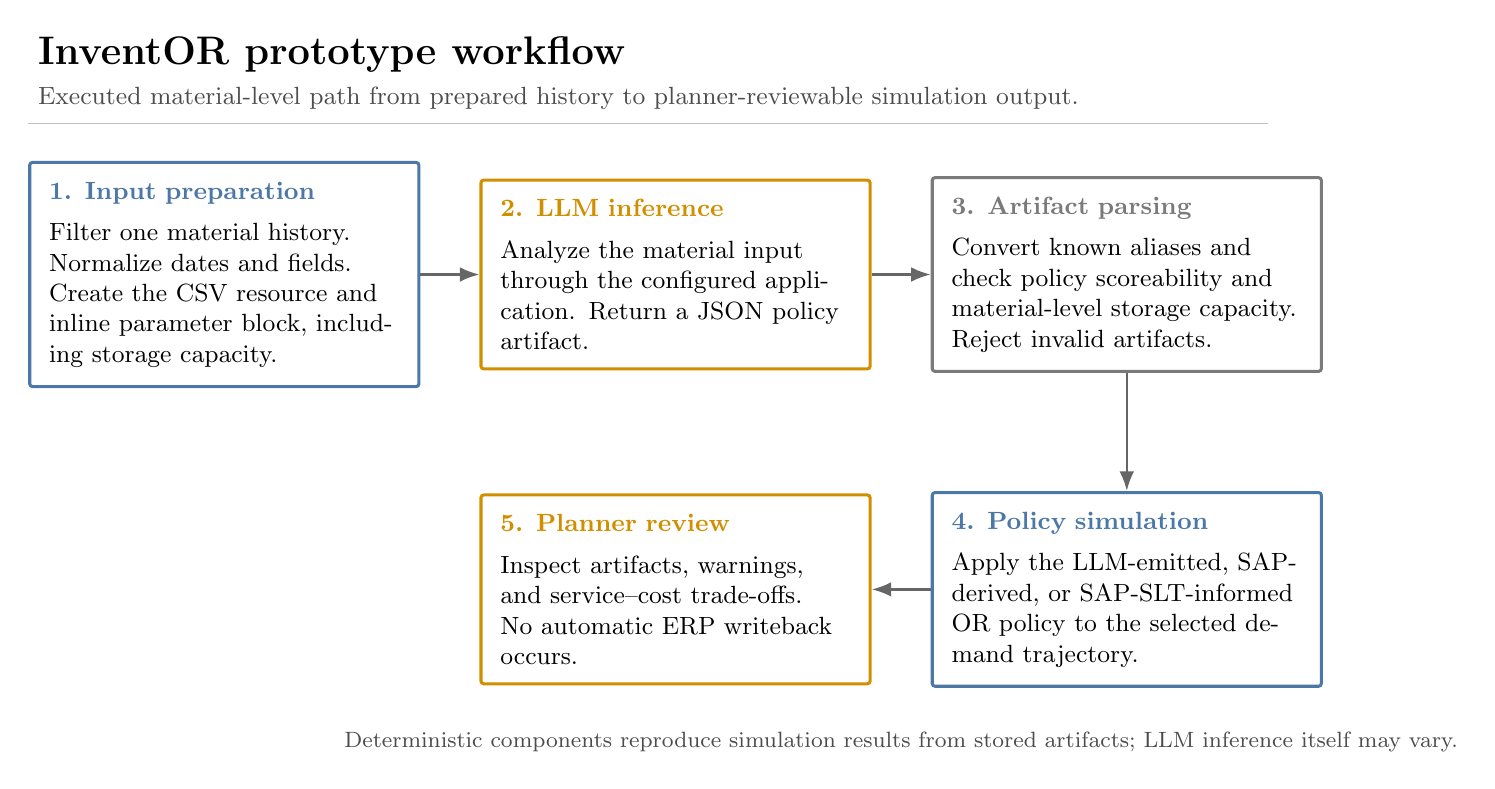
\begin{tikzpicture}[
  >=Latex,
  flow/.style={-Latex,draw=black!60,line width=0.9pt},
  box/.style={fill=white,line width=1.1pt,rounded corners=1pt,
    text width=4.45cm,minimum height=2.35cm,align=left,inner sep=7pt,
    font=\small},
  note/.style={font=\footnotesize,text=black!70,align=center}
]
\node[anchor=west,font=\Large\bfseries] at (0,0) {InventOR prototype workflow};
\node[anchor=west,font=\small,text=black!70] at (0,-0.55)
  {Executed material-level path from prepared history to planner-reviewable simulation output.};
\draw[black!25] (0,-0.88) -- (15.75,-0.88);

\node[box,draw=orblue,anchor=north west] (input) at (0,-1.35) {
  \textcolor{orblue}{\textbf{1. Input preparation}}\\[4pt]
  Filter one material history. Normalize dates and fields. Create the CSV resource and inline parameter block, including storage capacity.};

\node[box,draw=ororange,right=0.75cm of input] (llm) {
  \textcolor{ororange}{\textbf{2. LLM inference}}\\[4pt]
  Analyze the material input through the configured application. Return a JSON policy artifact.};

\node[box,draw=orgray,right=0.75cm of llm] (parse) {
  \textcolor{orgray}{\textbf{3. Artifact parsing}}\\[4pt]
  Convert known aliases and check policy scoreability and material-level storage capacity. Reject invalid artifacts.};

\node[box,draw=orblue,below=1.5cm of parse] (sim) {
  \textcolor{orblue}{\textbf{4. Policy simulation}}\\[4pt]
  Apply the LLM-emitted, SAP-derived, or SAP-SLT-informed OR policy to the selected demand trajectory.};

\node[box,draw=ororange,left=0.75cm of sim] (review) {
  \textcolor{ororange}{\textbf{5. Planner review}}\\[4pt]
  Inspect artifacts, warnings, and service--cost trade-offs. No automatic ERP writeback occurs.};

\draw[flow] (input.east) -- (llm.west);
\draw[flow] (llm.east) -- (parse.west);
\draw[flow] (parse.south) -- (sim.north);
\draw[flow] (sim.west) -- (review.east);

\node[note,anchor=north] at ($(review.south)!0.5!(sim.south)+(0,-0.45)$)
  {Deterministic components reproduce simulation results from stored artifacts; LLM inference itself may vary.};
\end{tikzpicture}
\end{document}
